% Revised by Zhuoran Zhang (andyzzr809@gmail.com) on May 2022 for a CMU CEE dissertation.
%====Originally from the CMU ECE dissertation template========
% For a more compact document, add the option openany to avoid starting all chapters on odd numbered pages
\documentclass[12pt, pdftex, openany]{cmu_cee_dissertation}

% This is a template for a CMU ECE dissertation.  It conforms to the
% requirements from ECE as of May 2013.  Most importantly, the title
% page is formatted as per ECE standards and does not contain the list
% of committee members.  This template was modified from cmuthesis.cls,
% published by David Koes (www.cs.cmu.edu/~dkoes).  The next comment
% block is from the original cmuthesis.cls file.

%This is a template for a CMU thesis.  It is 18 pages without any content :-)
% The source for this is pulled from a variety of sources and people.
% Here's a partial list of people who may or may have not contributed:
%
%        bnoble   = Brian Noble
%        caruana  = Rich Caruana
%        colohan  = Chris Colohan
%        jab      = Justin Boyan
%        josullvn = Joseph O'Sullivan
%        jrs      = Jonathan Shewchuk
%        kosak    = Corey Kosak
%        mjz      = Matt Zekauskas (mattz@cs)
%        pdinda   = Peter Dinda
%        pfr      = Patrick Riley
%        dkoes = David Koes
%        rajas = Raja Sambasivan

% David Koes's mmain contribution was putting everything into a single
% class files and small template.  Raja Sambasivan updated the
% template and also changed it so as to conform to ECE standards.

% rajas: include just packages I think are probably necessary...
\usepackage{amsmath}
\usepackage{multirow}
\usepackage{multicol}
\usepackage{algorithm2e}
\usepackage{color}
\usepackage{url}
\usepackage{bigfoot}
\usepackage{setspace}
  \onehalfspacing
% \usepackage[textwidth=0.9in, textsize=small, shadow, disable]{todonotes}
\usepackage{sectsty}
   \allsectionsfont{\sffamily}
\usepackage{totcount}
   \regtotcounter{chapter}

\ifx\pdfoutput\undefined
  % we are running LaTeX, not pdflatex
  \usepackage{graphicx}
\else
% we are running pdflatex, so convert .eps files to .pdf
  \def\pdfshellescape{1}
  \usepackage[pdftex]{graphicx}
  \usepackage{epstopdf}
  \usepackage[protrusion=true,expansion=true]{microtype}
\fi

% \usepackage[numbers, square, comma, sort]{natbib}
\usepackage{natbib}

% rajas: For a beautiful dissertation, use Minion Pro and Myriad Pro
% as default fonts.  If you have these fonts installed, uncomment the
% lines below.  If not, the fonts can be installed by following the
% directions at: 
% Minion Pro: 
%   * http://kieranhealy.org/blog/archives/2012/11/10/installing-minion-pro/
%   * http://jklukas.blogspot.com/2010/02/installing-minionpro-tex-package.html
% Myriad Pro: 
%   * http://www.gaehrken.de/fonts/MyriadPro.txt
\usepackage[T1]{fontenc}
\usepackage{textcomp}
%\usepackage{MinionPro}
%\usepackage{MnSymbol}
%\usepackage{MyriadPro}
%\renewcommand{\sfdefault}{MyriadPro-LF}

% \usepackage[letterpaper,twoside,inner=1.3in,outer=1.3in,bottom=1.3in,top=1.3in]{geometry}

\usepackage[letterpaper,twoside,inner=1.25in,outer=1.25in,bottom=1in,top=1in]{geometry}

\usepackage[%
  hypcap=true,
  font=small,
  labelfont=bf
]{caption}
\usepackage[hypcap=true]{subcaption}
\usepackage[%
  pdftex,             % using pdftex
  pagebackref=false,   % backreferences
  pageanchor=true,
  plainpages=false, 
  pdfpagelabels, 
  bookmarks,
  bookmarksnumbered,
  colorlinks=true,
  urlcolor=blue,
  filecolor=blue,
  linkcolor=black,
  citecolor=black,
  pdftitle={PhD thesis},
  pdfauthor={Zhuoran Zhang},
  pdfsubject={PhD thesis},
  pdfkeywords={},
  pdfproducer={pdfLaTeX},
  %pdfborder=0 0 0,  %removes outlines around hyper links in online display
]{hyperref}

% Add functions from my AMAR papers
%=================================================
%Basic
\usepackage{booktabs}
\usepackage{longtable}
\usepackage{threeparttable}
% \usepackage{subfigure}
\usepackage{multirow}
\usepackage{amsmath}
\usepackage{amsfonts}
\usepackage{amsthm}
\usepackage{soul} %highlight text
\usepackage{tabularx}
% \usepackage{ltablex}%long table with tabularx
% \usepackage{longtable}%long table with tabularx
\usepackage[normalem]{ulem}
\useunder{\uline}{\ul}{}
\usepackage{dcolumn }
% defines \RaggedRight
\usepackage{ragged2e}
\newcolumntype{L}[1]{>{\hsize=#1\hsize\RaggedRight} X}

%Figure and table caption
% \usepackage[labelfont=bf,justification=raggedright,singlelinecheck=false]{caption}
% \captionsetup[figure]{name=Fig. ,labelsep=period,justification=centering}
% \captionsetup[table]{labelsep=newline,font=footnotesize}
%Add support for line labels
% \usepackage{lineno,hyperref}
% \modulolinenumbers[5]

%Code-style text
\def\code#1{\texttt{#1}}

%Math equations
\newcommand{\reals}{\mathbb{R}}
\newcommand{\prox}{\operatorname{prox}}
\newcommand{\dom}{\operatorname{dom}}
\newcommand{\indep}{\perp \!\!\! \perp}
\def\R{\mathbb{R}}
\def\E{\mathbb{E}}
\def\P{\mathbb{P}}
\def\Cov{\mathrm{Cov}}
\def\Var{\mathrm{Var}}
\def\half{\frac{1}{2}}
\def\sign{\mathrm{sign}}
\def\supp{\mathrm{supp}}
\def\th{\mathrm{th}}
\def\tr{\mathrm{tr}}
\def\dim{\mathrm{dim}}
\def\hbeta{\hat{\beta}}

% Assumption format https://tex.stackexchange.com/questions/177256/reference-to-assumptions
\newtheorem{asu}{Assumption}
\newcounter{subassumption}[asu]
\renewcommand{\thesubassumption}{(\textit{\roman{subassumption}})}
\makeatletter
\renewcommand{\p@subassumption}{\theasu}% Counter prefix.
\makeatother
\newcommand{\subasu}{% Just like \item in a list, but for an asu
  \refstepcounter{subassumption}%
  \thesubassumption~\ignorespaces}

%========================================
% End functions from my AMAR papers

%Add glossaries of terms
\usepackage[]{glossaries}

% Make backreferences in the bibliography pretty
% \usepackage[hyperpageref]{backref} 
%    \renewcommand*{\backref}[1]{}  
%    \renewcommand*{\backrefalt}[4]{
%       \ifcase #1 
%          Not cited.
%       \or
%          Cited on page #2.
%       \else
%          Cited on pages #2.
%       \fi}

% The following margin commands are needed by \todonotes
% \setlength{\marginparwidth}{1.5cm}
% \setlength{\marginparsep}{1cm}

% Prevent latex from splitting footnotes across many pages
%\interfootnotelinepenalty=9999

% Provides a draft mark at the top of the document. 
% \draftstamp{\today}{DRAFT}

%Add glossaries of terms

\makenoidxglossaries

\newglossaryentry{CMF}
{
    name=Crash Modification Factor,
    description={The Crash Modification Factor(CMF), represents the relative change in
    crash frequency due to a change in one specific condition, when all other conditions and site characteristics remain constant}
}

\newglossaryentry{CMFunction}
{
    name=Crash Modification Function,
    description={The Crash Modification Function(CMFunction), represents the 
    the potential variation (heterogeneity) of CMFs amongst different subpopulations (e.g., in this dissertation, the subpopulations could be work zones with different roadway characteristics)}
}

\newglossaryentry{HSM}
{
    name=Highway Safety Manual,
    description={The Highway Safety Manual (HSM), published by the American Association of State Highway Transportation Officials (AASHTO) is the recognized source of information and methods for quantitatively evaluating traffic safety performance on existing or proposed roadways}
}


\newglossaryentry{ATE}
{
    name=average treatment effect,
    description={The difference in mean (average) outcomes between units assigned to the treatment and units assigned to the
    control}
}

\newglossaryentry{HTE}
{
    name=heterogeneous treatment effect,
    description={The difference in mean (average) outcomes between units assigned to the treatment and units assigned to the
    control, across different subgroups}
}


\begin{document} 

\frontmatter

%initialize page style, so contents come out right (see bot) -mjz
\pagestyle{empty}

\title{\bf \textsf{A CMU CEE dissertation}}
\author{Someone}
\date{August}
\Year{2022}
% \trnumber{XXX-XXXX}

\degrees{
B.S., XX, XX University, 2017\\
B.S., XX, XX University, 2017\\
}

\support{}
\disclaimer{}

% copyright notice generated automatically from Year and author.
% permission added if \permission{} given.

% \keywords{}
\maketitle

% \begin{dedication}
% To my dog.
% \end{dedication}

% \begin{keywordspage}
% \end{keywordspage}
\pagestyle{plain} % for toc, was empty

\clubpenalty=9999
\widowpenalty=9999

\begin{acknowledgments}

  Acknowledgements.


\end{acknowledgments}

\begin{abstract}

Abstract

\end{abstract}

\tableofcontents

\begin{listoftablesenv}
   \listoftables
\end{listoftablesenv}

\begin{listoffiguresenv}
   \listoffigures
\end{listoffiguresenv}

\begin{glossaryoftermsenv}
  
\clearpage
% \glsaddall
\printnoidxglossaries

\end{glossaryoftermsenv}

\mainmatter

%% Double space document for easy review:
% \renewcommand{\baselinestretch}{1.66}\normalsize

\chapter{Introduction}
\label{sec:chapter-introduction}


\begin{itemize}
  \item Example reference:
  \citep{zhangInferringCausalEffect2022,zhangEstimatingHeterogeneousTreatment2022,zhang2023effective};
  \citet{zhangInferringCausalEffect2022}.
  \item Example cross reference: Section~\ref{sec:chap1-motivation}
\end{itemize}

\hypertarget{Test}{%
  \section{Example cross-reference}\label{sec:chap1-motivation}}



\hypertarget{chap1-def-cmf}{%
  \subsection{Example subsection}\label{sec:chap1-def-cmf}}

Example terms: \Gls{HSM} 

Example equation:
  
\begin{equation}
    N_{predicted} = N_{SPF_{x}} \times \left( CMF_{1x} \times CMF_{2x} \times \ldots CMF_{yx} \right) \times C_{x}
\label{eq:chap1-cmf}
\end{equation}

Example cross-reference of equation: Equation~\ref{eq:chap1-cmf}.

Example table:

% Please add the following required packages to your document preamble:
% \usepackage{booktabs}
% \usepackage{multirow}
% \usepackage{graphicx}
\begin{table}[]
  \scriptsize
  \caption{A review on crash risk association with work zone configurations (1) }\label{tbl:rq1--review-deploy-1}
  % \resizebox{\textwidth}{!}{%
  \begin{tabularx}{\linewidth}
    % {XXXcccccc}
    % {XXXXXXXXX}
    {L{1.6}
    L{1.6}
    L{1.1}
    L{0.9}
    L{0.8}
    L{0.5}
    L{0.9}
    L{0.8}
    L{0.9}}
    % {p{2.5cm}p{2.5cm}p{1cm}p{0.7cm}p{0.7cm}p{0.7cm}p{0.7cm}p{0.7cm}p{1.2cm}}
    \toprule
    \multirow{2}{*}{Study}                                &
    \multirow{2}{*}{Model}                                &
    \multirow{2}{*}{Regression}                           &
    \multicolumn{3}{l}{Normalization of crash counts}     &
    \multicolumn{3}{l}{Work zone configurations}                        \\ \cmidrule(l){4-9}
                                                          &
                                                          & equations
                                                          & Duration  &
    Length                                                &
    VMT                                                   &
    Duration                                              &
    Length                                                &
    Closure setting                                                     \\ \cmidrule(r){1-9} 
    \citep{grahamAccidentSpeedStudies1977}                &
    Linear regression                                     &
    (1)                                                   &
                                                          &
                                                          &
    X                                                     &
    -                                                     &
    -                                                     &
    Y                                                                   \\
    \citep{garberAccidentCharacteristicsConstruction1990} &
    Linear regression                                     &
    (2)                                                   &
                                                          &
                                                          &
    X                                                     &
    +                                                     &
    +*                                                    &
    \textbackslash{}                                                    \\
    \citep{ullmanTrafficSafetyEvaluation2008}             &
    Empirical Bayesian                                    &
    \textbackslash{}                                      &
                                                          &
    X                                                     &
                                                          &
    \textbackslash{}                                      &
    \textbackslash{}                                      &
    Y                                                                   \\
    \citep{ozturkEstimatingImpactWork2014a}               &
    Negative binomial                                     &
    (2)                                                   &
    X                                                     &
                                                          &
                                                          &
    \textbackslash{}                                      &
    +                                                     &
    \textbackslash{}                                                    \\
    \citep{yangModelingCrashRisk2015}                     &
    Rare event logistic                                  &
    (1)                                                   &
    X                                                     &
                                                          &
                                                          &
    0                                                     &
    +                                                     &
    Y                                                                   \\
    \citep{chenModelingSafetyHighway2014}                 &
    Random effect negative binomial                       &
    (1)                                                   &
    X                                                     &
                                                          &
                                                          &
    \textbackslash{}                                      &
    +                                                     &
    Y                                                                   \\
    \citep{yangModelingWorkZone2013}                      &
    Negative binomial with   measurement error            &
    (1)                                                   &
    X                                                     &
                                                          &
                                                          &
    \textbackslash{}                                      &
    +                                                     &
    Y                                                                   \\
    \citep{ozturkCrashFrequencyModeling2013b}             &
    Negative binomial                                     &
    (1)                                                   &
    X                                                     &
                                                          &
                                                          &
    +                                                     &
    +                                                     &
    Y                                                                   \\
    \citep{qiFrequencyWorkZone2005}                      &
    Truncated negative binomial and   Poisson             &
    (1)                                                   &
                                                          &
                                                          &
                                                          &
    +                                                     &
    +                                                     &
    Y                                                                   \\
    \citep{khattakEffectsWorkZone2002}                    &
    Negative binomial                                     &
    (2)                                                   &
    X                                                     &
                                                          &
                                                          &
    +                                                     &
    +                                                     &
    \textbackslash{}                                                    \\
    \citep{venugopalSafetyModelsRural2000}                &
    Negative binomial                                     &
    (1)                                                   &
                                                          &
                                                          &
                                                          &
    +                                                     &
    +                                                     &
    Y                                                                   \\
    \citep{palAnalysisCrashRates1996}                     &
    Negative binomial and Poisson                         &
    (1)                                                   &
                                                          &
                                                          &
    X                                                     &
    +                                                     &
    +                                                     &
    Y                                                                   \\
    \citep{latorreEffectsStationaryWork2017a}             &
    Empirical Bayesian                                    &
    \textbackslash{}                                      &
    X                                                     &
                                                          &
                                                          &
    \textbackslash{}                                      &
    \textbackslash{}                                      &
    Y                                                                   \\
    \citep{srinivasanUseEmpiricalBayesian2011}            &
    Empirical Bayesian                                    &
    \textbackslash{}                                      &
    X                                                     &
                                                          &
                                                          &
    \textbackslash{}                                      &
    \textbackslash{}                                      &
    Y                                                                   \\ \bottomrule
  \end{tabularx}%
  % }

  \vspace{2ex}
  {\footnotesize Notes: ``+'' positive effect, ``-'' negative effect, ``0'' no significant changes, ``\textbackslash{}'' not applicable ``Y'' associated, ``N'' not associated; ``X'' used.\par
    *: \citet{garberAccidentCharacteristicsConstruction1990} found work zone crash risk decreased with increase in work zone length for work zone lengths up to 0.6 mile, and work zone crash risk increased with increase in work zone length for work zone lengths longer than 0.6 mile.
    \par}
\end{table}


Table~\ref{tbl:rq1--review-deploy-1} provides an overview of prior studies on deriving associations
of work zone configurations with work zone crash risks. 


\begin{figure}[h]
  \centering
  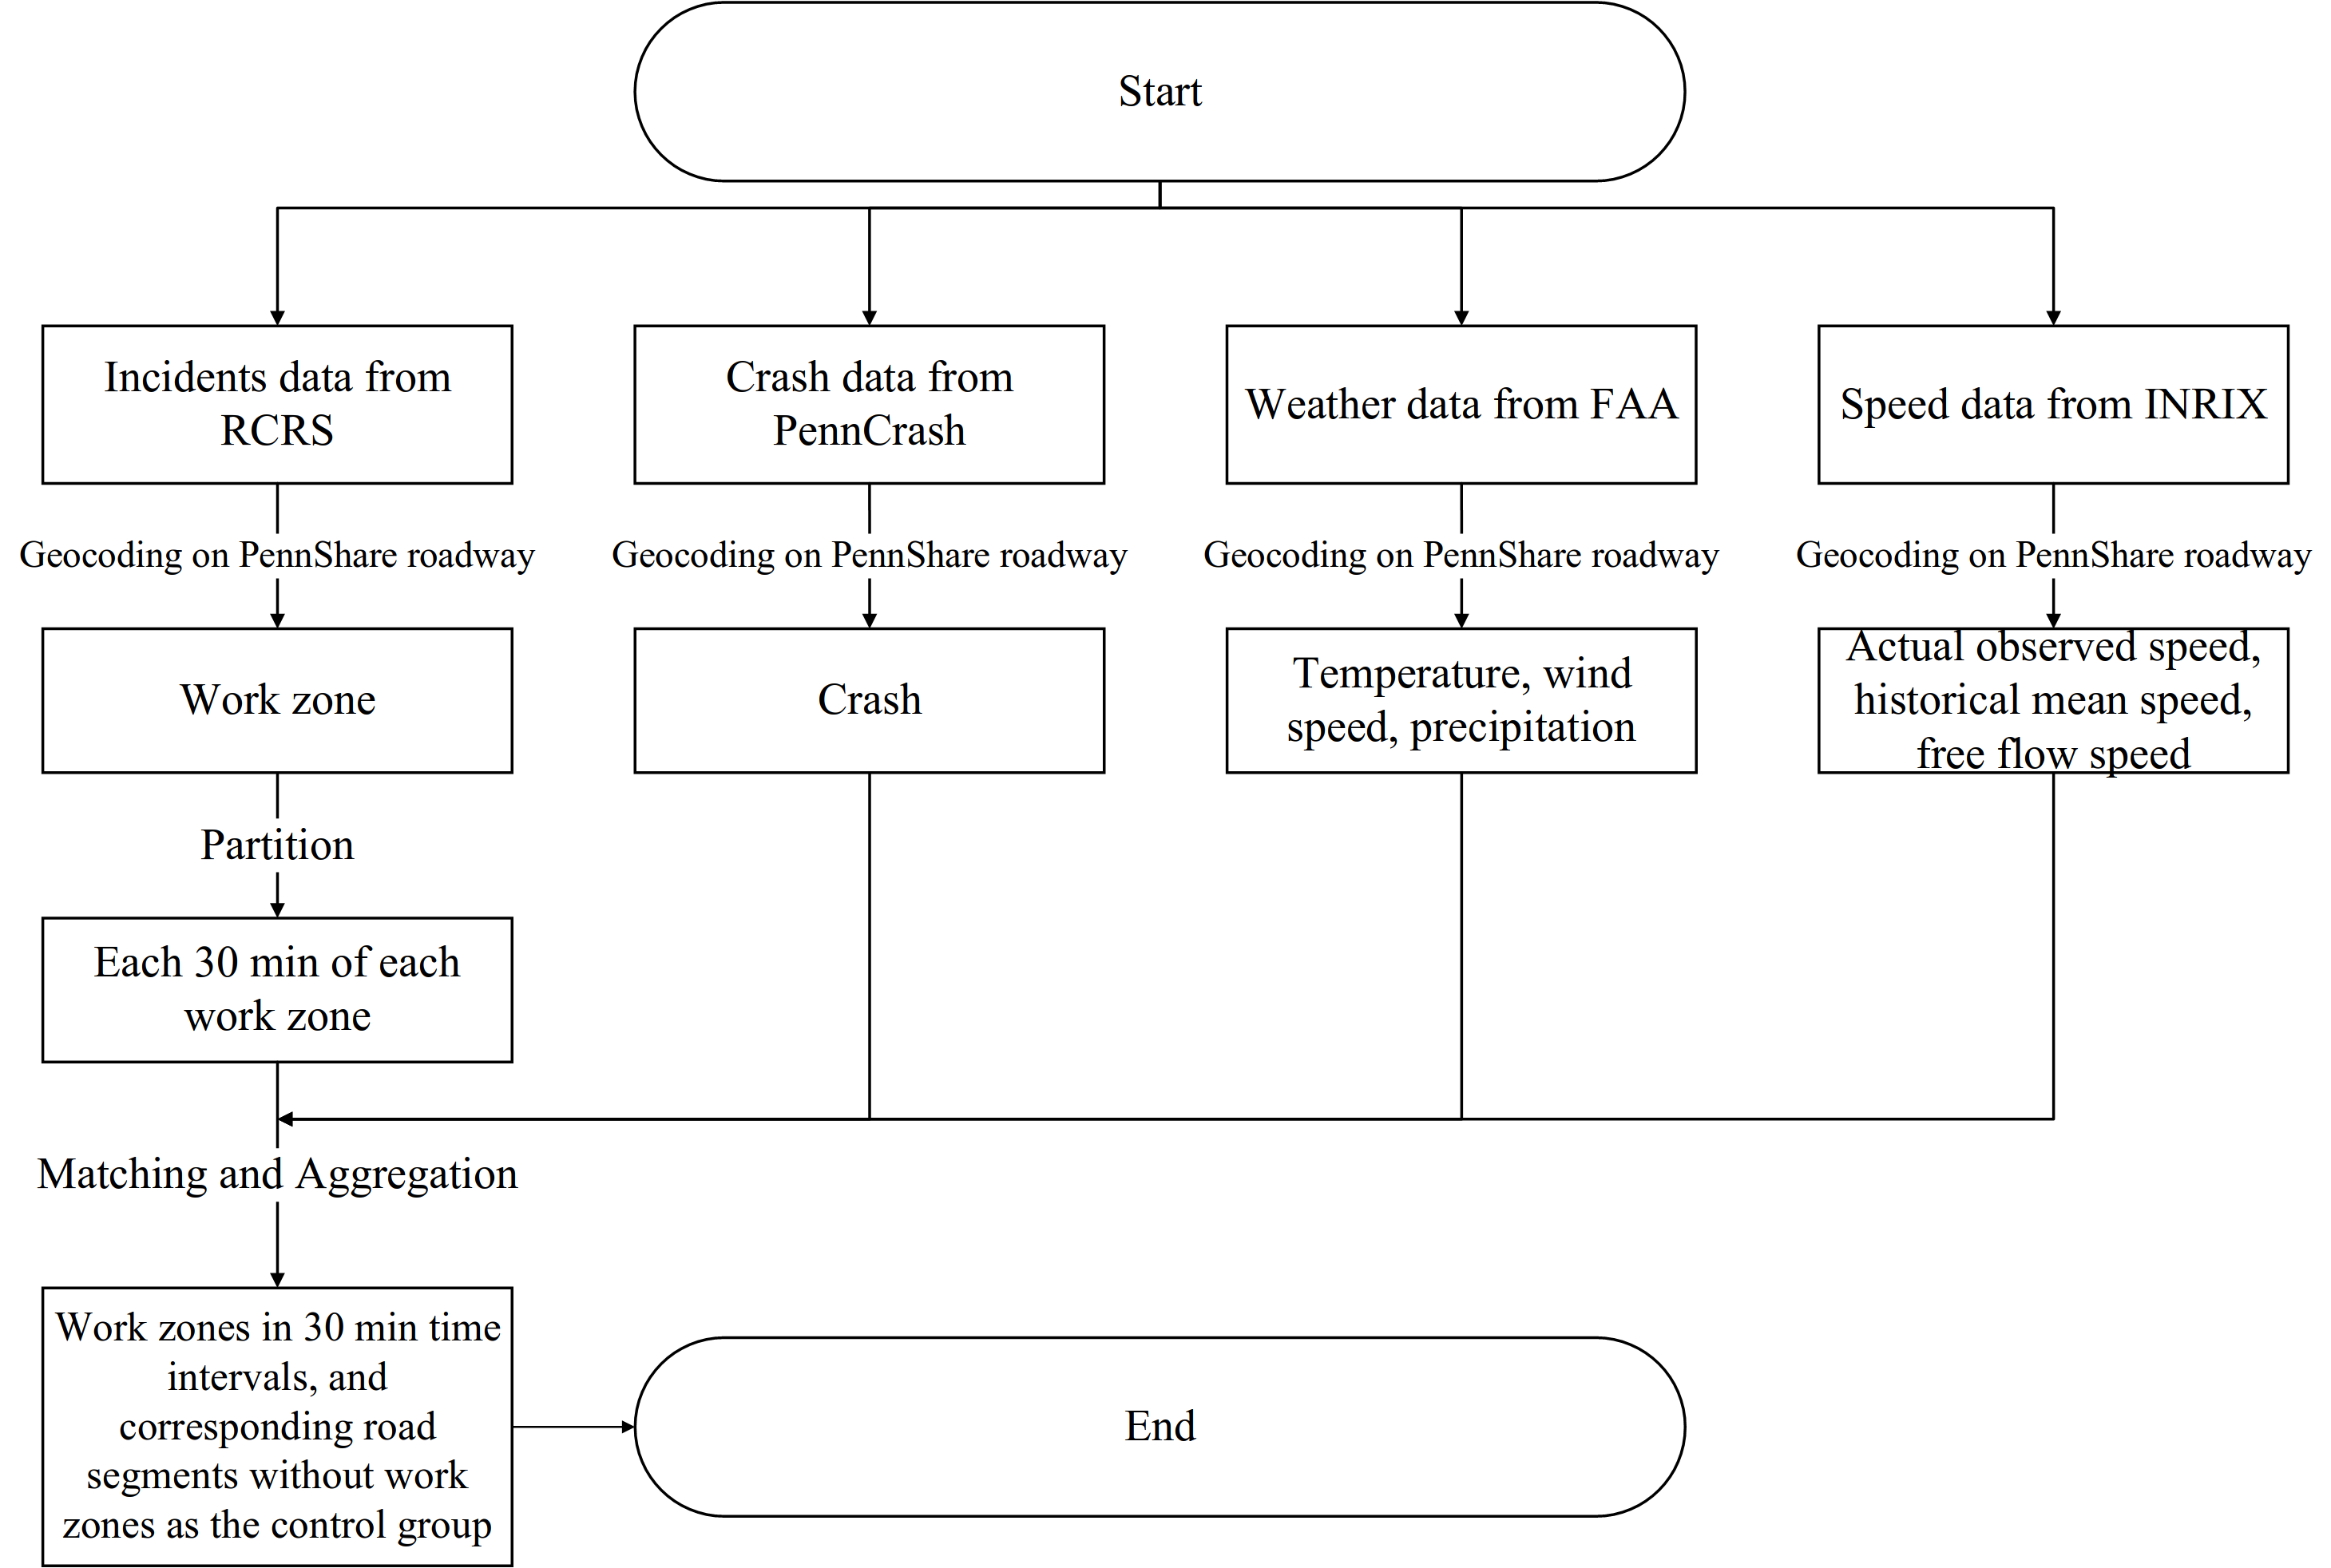
\includegraphics[width=1\textwidth]{media/rq1/DataProcessing3.png}
  \caption{Data processing workflow}\label{fig:rq1-1:dataprocessingflow}
\end{figure}

Figure~\ref{fig:rq1-1:dataprocessingflow} presents the workflow of data processing.
  



\backmatter

%\renewcommand{\baselinestretch}{1.0}\normalsize
% By default \bibsection is \chapter*, but we really want this to show
% up in the table of contents and pdf bookmarks.
\renewcommand{\bibsection}{\chapter{\bibname}}
%\setlength\bibsep{0pt plus 1pt}
%\newcommand{\bibpreamble}{This text goes between the ``Bibliography''
%  header and the actual list of references}
\bibliographystyle{ascelike}
\bibliography{Zoterobib} %your bib file
\end{document}
